\documentclass{CPSReport}

\setminted[python3]{breaklines, framesep=2mm, fontsize=\footnotesize, numbersep=5pt}
\usemintedstyle{friendly}

%----------------------------------------------------------------------------------------
%	AUTHOR / TITLE INFORMATION
%----------------------------------------------------------------------------------------
\title{Assignment V: Non-Linear Probabilistic Regression Models} % The article title

\author{
	\coursetitle{Introduction to Machine Learning Lab (190.013), SS2023}
	\authorstyle{Björn Ellensohn\textsuperscript{1}} % Authors
	\newline\newline % Space before institutions
	\textsuperscript{1}\textit{m01435615}, \textit{bjoern.ellensohn@stud.unileoben.ac.at}, \institution{Montanuniversität Leoben, Austria}\\ % Institution 1
	\submissiondate{\today} % Add a date here
}

%----------------------------------------------------------------------------------------
%	DOCUMENT
%----------------------------------------------------------------------------------------

\begin{document}

\maketitle % Print the title

\thispagestyle{firstpage} % Apply the page style for the first page (no headers and footers)

%----------------------------------------------------------------------------------------
%	ABSTRACT
%----------------------------------------------------------------------------------------

\lettrineabstract{This document guides through the process of solving Assignment 5.}

\section{Introduction}
The 5$^{th}$ assignment's task offers us with a more advanced look at machine learning techniques. This time it was allowed to use scikit-learn which makes life much easier for a data scientist. So it is even possible to directly import datasets from scikit library. In this assignment, we are evaluating the "iris" dataset from scikit-learn and the "concrete" dataset from UCI.  In the end, the algorithms that had to be integrated where:
\begin{itemize}
    \item Perceptron Algorithm
    \item Polynomial Regression
    \item Radial Basis Functions Regression
    \item Multilayer Perceptron Algorithm (Bonus)
\end{itemize}

I will walk through the code in 4 Sections.

\section{Part I - Perceptron Algorithm}
\subsection{First Things First}
As a guide through the assignment, an unsolved Jupyter Notebook was given, so we had an outline on how to solve this task. Before the actual code starts, dependencies had to be installed via \mintinline{python}{pip install}. Also, the iris dataset is loaded from scikit-learn via \mintinline{python}{load_iris()}. 

\subsection{Preparing the Data}
Data preprocessing is an essential part of machine learning tasks. The dataset has to be examined for outliers and missing values. Outliers can easily be found using \mintinline{python}{DataFrame.boxplot()} and doing a 1.5 x IQR analysis. Outliers and missing values are then mitigated by selecting an approach which must be adapted to the type of data given. One simple method is replacing the outlier or missing data with the mean value of the column. After that is done, the dataset must be split into features and targets, which are in turn separated into training and testing sets. So in the end we will end up with four datasets:
\begin{itemize}
    \item X\_train
    \item X\_test
    \item y\_train
    \item y\_test
\end{itemize}
Where the *class\_train sets are used to evaluate the performance of the regression methods later.

\subsection{Defining the Perceptron Algorithm}
The Perceptron Algorithm, is the most basic single-layered neural network used for binary classification. This algorithm was inspired by the basic processing units in the brain, called neurons, and how they process signals. A visualization as of how the model works is seen in Figure~\ref{fig:perceptron}.
\begin{figure}[ht]
    \centering
    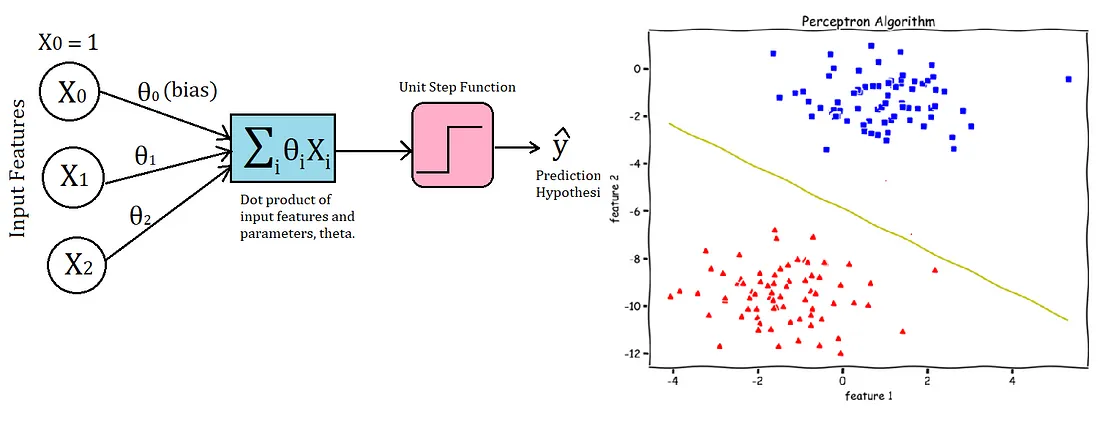
\includegraphics[width=.9\linewidth]{pics/perceptron.png}
    \caption{Perceptron Algorithm Description.}
    \label{fig:perceptron}
\end{figure}

The formula for the Perceptron update rule is displayed in Figure~\ref{fig:form_perceptron}.
\begin{figure}[ht]
    \centering
    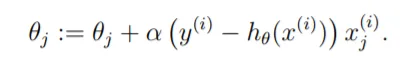
\includegraphics[width=0.9\linewidth]{pics/perceptron_formula.png}
    \caption{The Formula for Perceptron Algorithm.}
    \label{fig:form_perceptron}
\end{figure}

For the implementation in Python a class \mintinline{python}{MultiClassPerceptron} is created which takes as inputs the input dimensions of provided data, the wanted output dimensions, the learning rate and the number of epochs. The forward, backward and predict functions had to be implemented.

In this implementation, the forward() method calculates the weighted sum of inputs and biases, applies the softmax function to obtain class probabilities, and returns the probabilities. The backward() method calculates the gradients of the weights and biases using the predicted probabilities and the true labels, and then updates the parameters using gradient descent. The predict() method uses the forward() method to get the class probabilities and selects the class with the highest probability as the predicted class for each example.

\subsubsection{Forward Function}
\begin{minted}{python3}
    def forward(self, X):
        weighted_sum = np.dot(X, self.W) + self.b
        probabilities = np.exp(weighted_sum) / np.sum(np.exp(weighted_sum), axis=1, keepdims=True)
        return probabilities
\end{minted}

\subsubsection{Backward Function}
\begin{minted}{python3}
    def backward(self, X, y):
        m = X.shape[0]

        probabilities = self.forward(X)
        # Convert y to one-hot encoded form
        y_one_hot = np.eye(self.W.shape[1])[y]

        dW = (1 / m) * np.dot(X.T, (probabilities - y_one_hot))
        db = (1 / m) * np.sum(probabilities - y_one_hot, axis=0)

        self.W -= self.lr * dW
        self.b -= self.lr * db
\end{minted}

\subsubsection{Predict Function}
\begin{minted}{python3}
    def predict(self, X):
        probabilities = self.forward(X)
        predictions = np.argmax(probabilities, axis=1)
        return predictions
\end{minted}

\subsection{Evaluation}
Having the code done, the model is then be trained and evaluated. For performance analysis, accuracy\_score method from the scikit-learn metrics package is used. Having tuned the lr parameter to 0.0005 the Perceptron classification train accuracy is 0.6666666666666666 and the Perceptron classification accuracy is 0.7. However, when re-running the training, the results change so I assume there must be a problem somewhere.

\FloatBarrier
\section{Part II - Polynomial Regression}
\subsection{Introduction}
If your data points are not connectable by a straight line, Polynomial Regression might help you out. Figure~\ref{fig:example_poly} gives a nice example how this looks like.
\begin{figure}[ht]
    \centering
    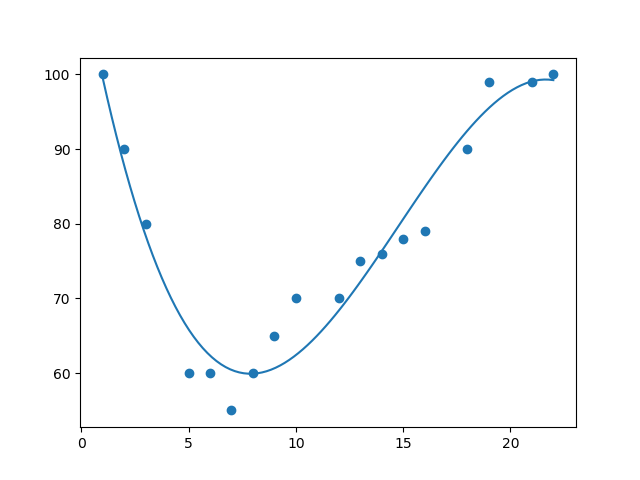
\includegraphics[width=0.9\linewidth]{pics/polynomial_regression_example.png}
    \caption{Exemplary Display of Polynomial Regression.}
    \label{fig:example_poly}
\end{figure}

\subsection{Preparing the Data}
This time, the "concrete" dataset from UCI shall be processed and evaluated. Since the data is provided in an xls file, it must first be imported into a Pandas dataframe. After that, the usual feature and target selection is taking place. The concrete's compressive strength is selected as target, as this is connected to all the other parameters of this dataset. So the other columns are threated as features. In the code, this is achieved by using the \mintinline{python}{DataFrame.drop()} method and slicing.

\subsection{Implementing the Polynomial Regression}
The data preparation part once again leads to four subsets:
\begin{itemize}
    \item X\_train
    \item X\_test
    \item y\_train
    \item y\_test
\end{itemize}

Next, the features had to be transformed into polynomials. This is done using a hand-made function called \mintinline{python}{polynomial_features()}, which takes as inputs the desired polynomial's degree and the subset to process.

The function iterates over the combinations with replacement of feature indices up to the specified degree using \mintinline{python}{combinations_with_replacement()}. For each combination, it creates a new array of polynomial features by multiplying the corresponding columns of X. The resulting polynomial features are appended to the \mintinline{python}{polynomial_X} list.

Finally, the list of polynomial features is stacked horizontally using \mintinline{python}{np.column_stack()} to form the final \mintinline{python}{polynomial_X} array, which is then returned. The code for that follows.

\subsubsection{Polynomial Features Function}
\begin{minted}[breakanywhere=true,breaklines]{python3}
    def polynomial_features(X, degree):
    n_samples, n_features = X.shape
    polynomial_X = np.ones((n_samples, 1))

    for d in range(1, degree + 1):
        combinations = combinations_with_replacement(range(n_features), d)
        for comb in combinations:
            poly_features = np.prod(X[:, comb], axis=1, keepdims=True)
            polynomial_X = np.hstack((polynomial_X, poly_features))

    return polynomial_X
\end{minted}

\subsubsection{Training the Model}
After that, the LinearRegression class from sklearn.linear\_model is used to make life easier but we will extend it by using our \mintinline{python}{polynomial_features()}. Now we are almost ready to train our model, only some minor steps need to be taken. Let's see the code:
\begin{minted}{python3}
    # Train the model
    lr_poly_custom = LinearRegression()
    lr = LinearRegression()
    # fit the model
    lr_poly_custom.fit(X_train_poly_custom, y_train)
    lr.fit(X_train, y_train)
    # predict values from the polynomial transformed features
    predictions_poly_custom_train = lr_poly_custom.predict(X_train_poly_custom)
    predictions_poly_custom = lr_poly_custom.predict(X_test_poly_custom)
    # predict values from the original features
    predictions_train = lr.predict(X_train)
    predictions = lr.predict(X_test)
\end{minted}

\subsubsection{Evaluation}
To better get a feel for the Polynomial Regression's performance, it is also compared to a standard linear regression model on the same dataset. The results are displayed in Figure~\ref{fig:eval_poly}.
\begin{figure}[ht]
    \centering
    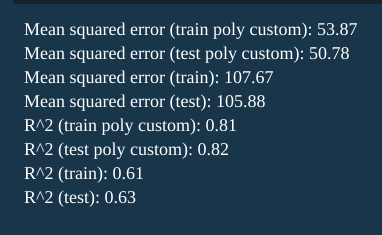
\includegraphics[width=0.9\linewidth]{pics/polynomial_eval.png}
    \caption{Evaluation of Polynomial Regression compared to Linear Regression.}
    \label{fig:eval_poly}
\end{figure}

Comparing the mean squared error values, it is easy to say that Polynomial Regression performance is way better in this case.
\clearpage

\section{Part III - Radial Basis Functions Regression}
Another way to implement non-linear Regression is using Radial Basis Functions (RBFs).
\subsection{Introduction}
For the vast variety of datasets out there it is always good to have some specialized regression models at hand.
The RBF Regression follows formula~\eqref{eq:radial}.
\begin{align}\label{eq:radial}
    h(x) = \sum_{n=1}^N w_n \times exp(-\gamma \|x-x_n\|^2)
\end{align}
A visualization of RBFs can be seen in figure~\ref{fig:RBFs}.
\begin{figure}[ht]
    \centering
    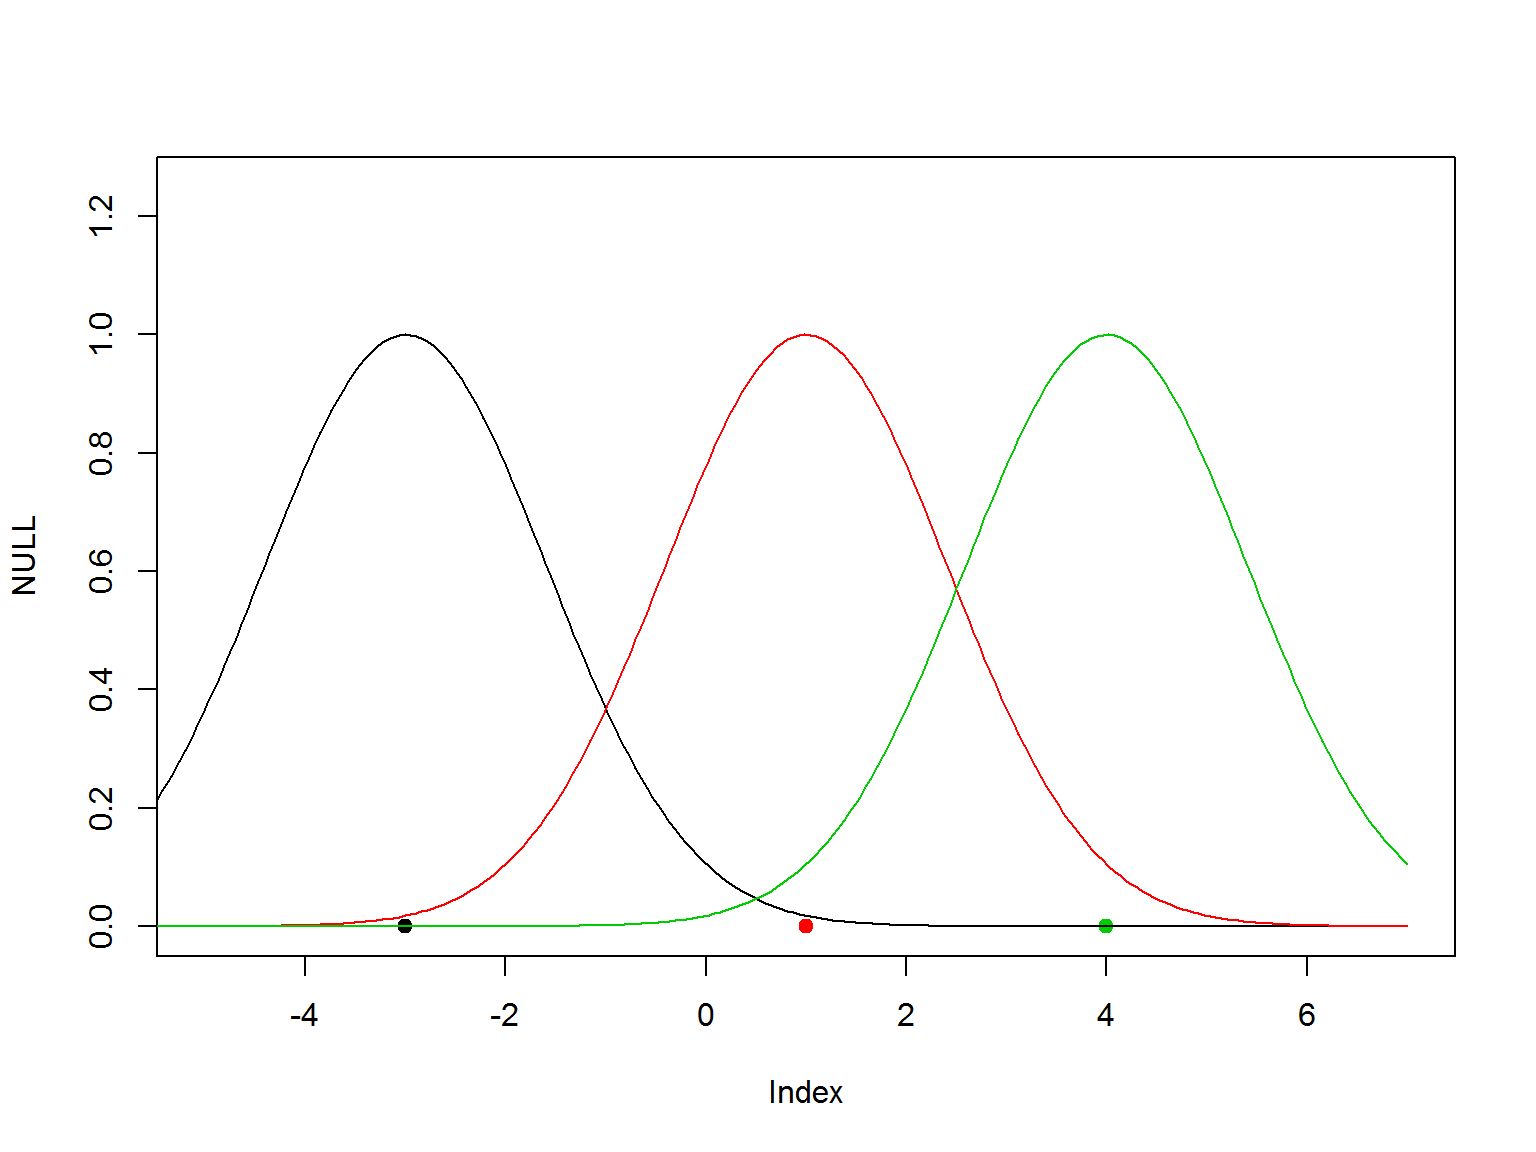
\includegraphics[width=0.9\linewidth]{pics/RBFs.png}
    \caption{Evaluation of Polynomial Regression compared to Linear Regression.}
    \label{fig:RBFs}
\end{figure}

\subsection{Walktrough RBFs}
For this part of the assignment, the California Housing Prices dataset is used. It is included into scikit-learn and can be imported by calling the \mintinline{python}{fetch_california_housing()} method.

Again, \mintinline{python}{train_test_split()} is used to produce some fine subsets for the following data-science-fun. As a preparation step the data standardized too. The \mintinline{python}{StandardScaler} class is best-suited for this kind of work:
\begin{minted}{python3}
    scaler = StandardScaler()
    X_train_std = scaler.fit_transform(X_train)
    X_test_std = scaler.fit_transform(X_test)
\end{minted}

The most important part was implementing the \mintinline{python}{rbf_kernel()} function so i print it right here:
\begin{minted}{python3}
def rbf_kernel(X, centers, gamma):
    n_samples = X.shape[0]
    n_centers = centers.shape[0]
    K = np.zeros((n_samples, n_centers))

    for i in range(n_samples):
        for j in range(n_centers):
            diff = X[i] - centers[j]
            K[i, j] = np.exp(-gamma * np.dot(diff, diff))

    return K
\end{minted}

The remaining steps are as following. As always, the full code is attached in the appendix, so a short summary will do for now.
\begin{enumerate}
    \item Choose the number of centroids and the RBF kernel width
    \item Randomly select the centroids from the training set
    \item Compute the RBF features for the training and testing sets
    \item Fit a linear regression model on the original and RBF-transformed data
\end{enumerate}
After these steps, the evaluation could take place.

\subsection{Evaluation}
The RBF Regression is compared against the normal Linear Regression. To my surprise, the results only show a minor difference between those two methods. This is pictured in figure~\ref{fig:RBF_eval}. 
\begin{figure}[ht]
    \centering
    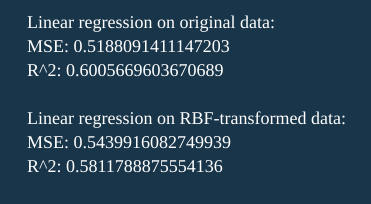
\includegraphics[width=0.9\linewidth]{pics/RBF_eval.png}
    \caption{Evaluation of RBF Regression compared to Linear Regression.}
    \label{fig:RBF_eval}
\end{figure}
\clearpage

\section{Part IV - Multilayer Perceptron Algorithm (Bonus)}
The bonus part was skipped so there is not much to say here.

\newpage
\onecolumn
\section*{APPENDIX}\label{sec:appendix}

The complete code is following.

\subsection*{Code for Part I}
\inputminted[%
breakanywhere=true,
breaklines,
mathescape,
linenos,
numbersep=5pt,
frame=single,
numbersep=5pt,
xleftmargin=0pt,
]{python3}{include/part1.py}

\subsection*{Code for Part II}
\inputminted[%
breakanywhere=true,
breaklines,
mathescape,
linenos,
numbersep=5pt,
frame=single,
numbersep=5pt,
xleftmargin=0pt,
]{python3}{include/part2.py}

\subsection*{Code for Part III}
\inputminted[%
breakanywhere=true,
breaklines,
mathescape,
linenos,
numbersep=5pt,
frame=single,
numbersep=5pt,
xleftmargin=0pt,
]{python3}{include/part3.py}

\newpage

\thispagestyle{lastpage}
\end{document}